\subsection{Software}
The entire system is controlled by a Raspberry Pi 4B running a very lightweight Linux distribution called DietPi\cite{dietpi}.
The goal for the entire system is to be run locally on the Pi, so the Pi will be responsible for running the computer vision system,
controlling the hardware, and running the user interface. In order to achieve this, the following software components are required:
\begin{mylist}
  \item The User Interface
  \item The Computer Vision system
  \item The Hardware Control system
\end{mylist}
\noindent
The system's software is written in Python\cite{python}, which is well suited for the project given the 
availability of libraries for computer vision and hardware control. Again, the concept of modularity underpins the design of the software,
and so each component is designed to be independent of the others and can be developed in parallel.

All written Python code adheres to a style defined in a .pylintrc file, which is a configuration file for the pylint\cite{pylint} linter. This ensures
that the code is consistent and readable. The code is also documented using docstrings for 
readability and maintainability. Each software component is designed to be self-contained so they can be run independently for testing purposes.

All software constants are defined in a constants.py file, which is imported by all other Python files, allowing for easy modification of constants
that define the behaviour of the system which is useful for testing and debugging.

Additionally, a lot of thought went into streamlining the development process to ensure that the system is easy to develop and maintain. For example,
Visual Studio Code's\cite{vscode} Remote SSH extension is used to develop the system remotely, as it allows developing the system on a much more powerful laptop, while
using the familiar VSCode environment with any extensions that help streamline the development process. This is crucial as the Pi is not very powerful, so
compiling and running the system on the Pi may be slow and cumbersome.

The Pi uses Git\cite{git} for version control, and the repository is hosted on GitHub\cite{github}, with a dedicated branch for the Pi that is regularly
updated with the main branch. The vision system and the laptop also maintain their own Git branches which are regularly updated with the main branch, ensuring 
that all systems are running the same code. This is crucial as it enables development on a more powerful laptop, and then synchronises the changes to the Pi, without
having to manually copy any files over.

During development, the Pi connects to the laptop's WiFi hotspot and is configured to be discoverable with the Pi's hostname, facilitating easy access to the Pi through
SSH and a VNC Viewer without needing the Pi's IP address, which is dynamic. The Pi also makes use of SSH keys, allowing connection 
to the Pi without needing to enter a password every time, ensuring quick and easy access.



% User Interface
\noindent
\textbf{User Interface} \\
As the system is intended to be self-contained, it is important to have a user interface that displays all relevant information to the user
and allows them to interact with the system. The UI is displayed on the 7" touchscreen display, and is written using Pygame\cite{pygamedoc};

This design decision was made after experimentation with other UI libraries like Tkinter\cite{tkinterdoc}, however it was found that Pygame was the most
viable for several reasons; it contains a module for camera streaming, which is used to display the camera feed on the UI, and can also be used to
feed the camera frames to the Computer Vision system; there is a very large amount of control provided by Pygame over the UI, especially in terms of 
performance. This is crucial as the UI is only there to provide information to the user, and so it must not interfere with the
computer vision system or the hardware control system. With an additional library named pygame\_gui\cite{pygamegui}, it is possible to create a UI with 
GUI elements like buttons, text boxes, and drop-down menus, making for a fully comprehensive UI library.

In Figure \ref{fig:mainui}, the current version of the UI is shown. On the left, the camera feed and camera frame rate are displayed, with the system
CPU and RAM usage displayed, for monitoring purposes. There is a slider to adjust the power of the connected LED Ring light, as well as two buttons
related to the Computer Vision system.

The right side is empty for now but will be used to display information about the computer vision system and the hardware control system.

\begin{figure*}[t]
  \begin{minipage}[t]{\textwidth}
    \centering
    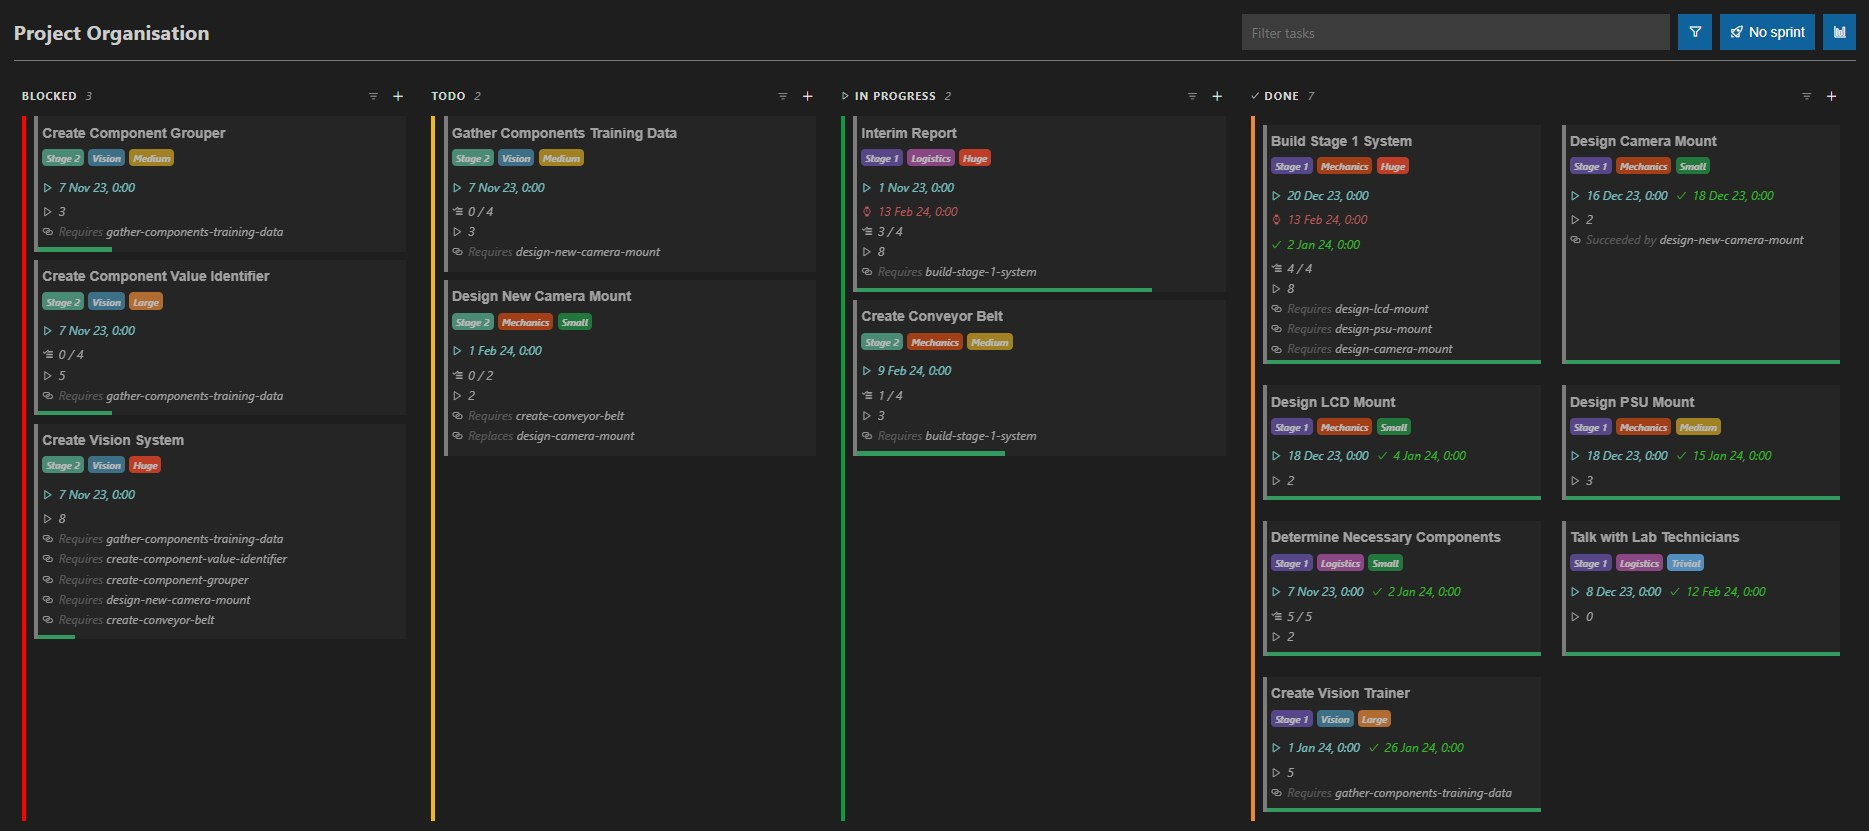
\includegraphics[width=\textwidth,height=10.5cm,keepaspectratio]{imgs/appendix/projectplan.jpg}
    \caption{Project Plan}
    \label{fig:projectplan}
  \end{minipage}
  \hfill 
\end{figure*}
